\chapter{PCB Specifications} % Main appendix title

\label{AppendixA} % For referencing this appendix elsewhere, use \ref{AppendixA}

\section{PCB Schematic}

\begin{figure}[h]
  \centering
  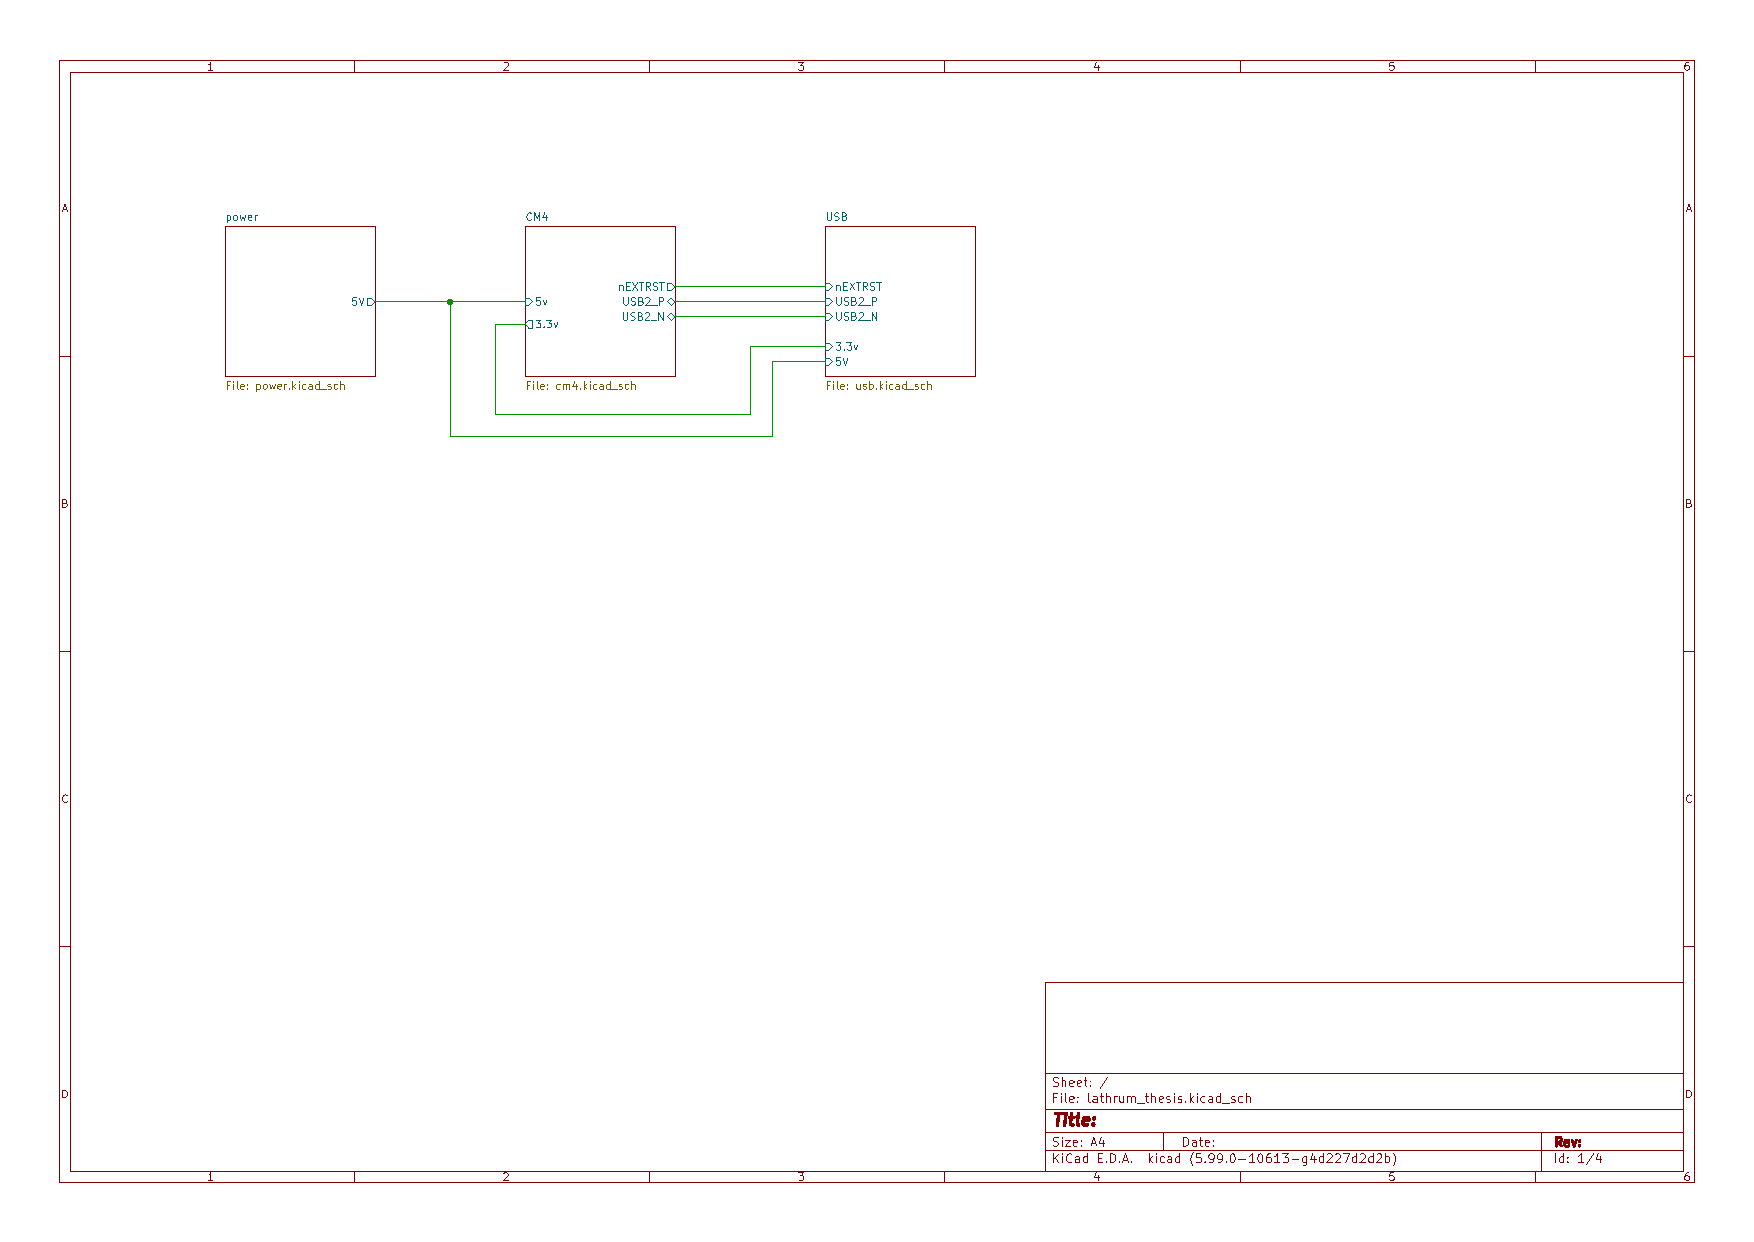
\includegraphics[width=1\textwidth,page=1]{Figures/kicad/lathrum_thesis_schematic.pdf}
  \captionsetup{width=.8\linewidth}
  \caption[Top Level Schematic]{The top level of the PCB board schematic}
  \label{fig:pcb_schematic_top}
\end{figure}

\begin{figure}[h]
  \centering
  \includegraphics[width=1\textwidth,page=2]{Figures/kicad/lathrum_thesis_schematic.pdf}
  \captionsetup{width=.8\linewidth}
  \caption[Power Schematic]{Schematic layout for the power circuit, including battery management}
  \label{fig:pcb_schematic_battery}
\end{figure}

\begin{figure}[h]
  \centering
  \includegraphics[width=1\textwidth,page=3]{Figures/kicad/lathrum_thesis_schematic.pdf}
  \captionsetup{width=.8\linewidth}
  \caption[CM4 Schematic]{Schematic layout for interfacing with the Compute Module 4}
  \label{fig:pcb_schematic_cm4}
\end{figure}

\begin{figure}[h]
  \centering
  \includegraphics[width=1\textwidth,page=4]{Figures/kicad/lathrum_thesis_schematic.pdf}
  \captionsetup{width=.8\linewidth}
  \caption[USB Schematic]{Schematic layout for the USB hub and ports}
  \label{fig:pcb_schematic_usb}
\end{figure}

% Make sure next section is on a new page
\clearpage
\section{PCB Layout}

\begin{figure}[h]
  \centering
  %Height instead of width because the image is rotated
  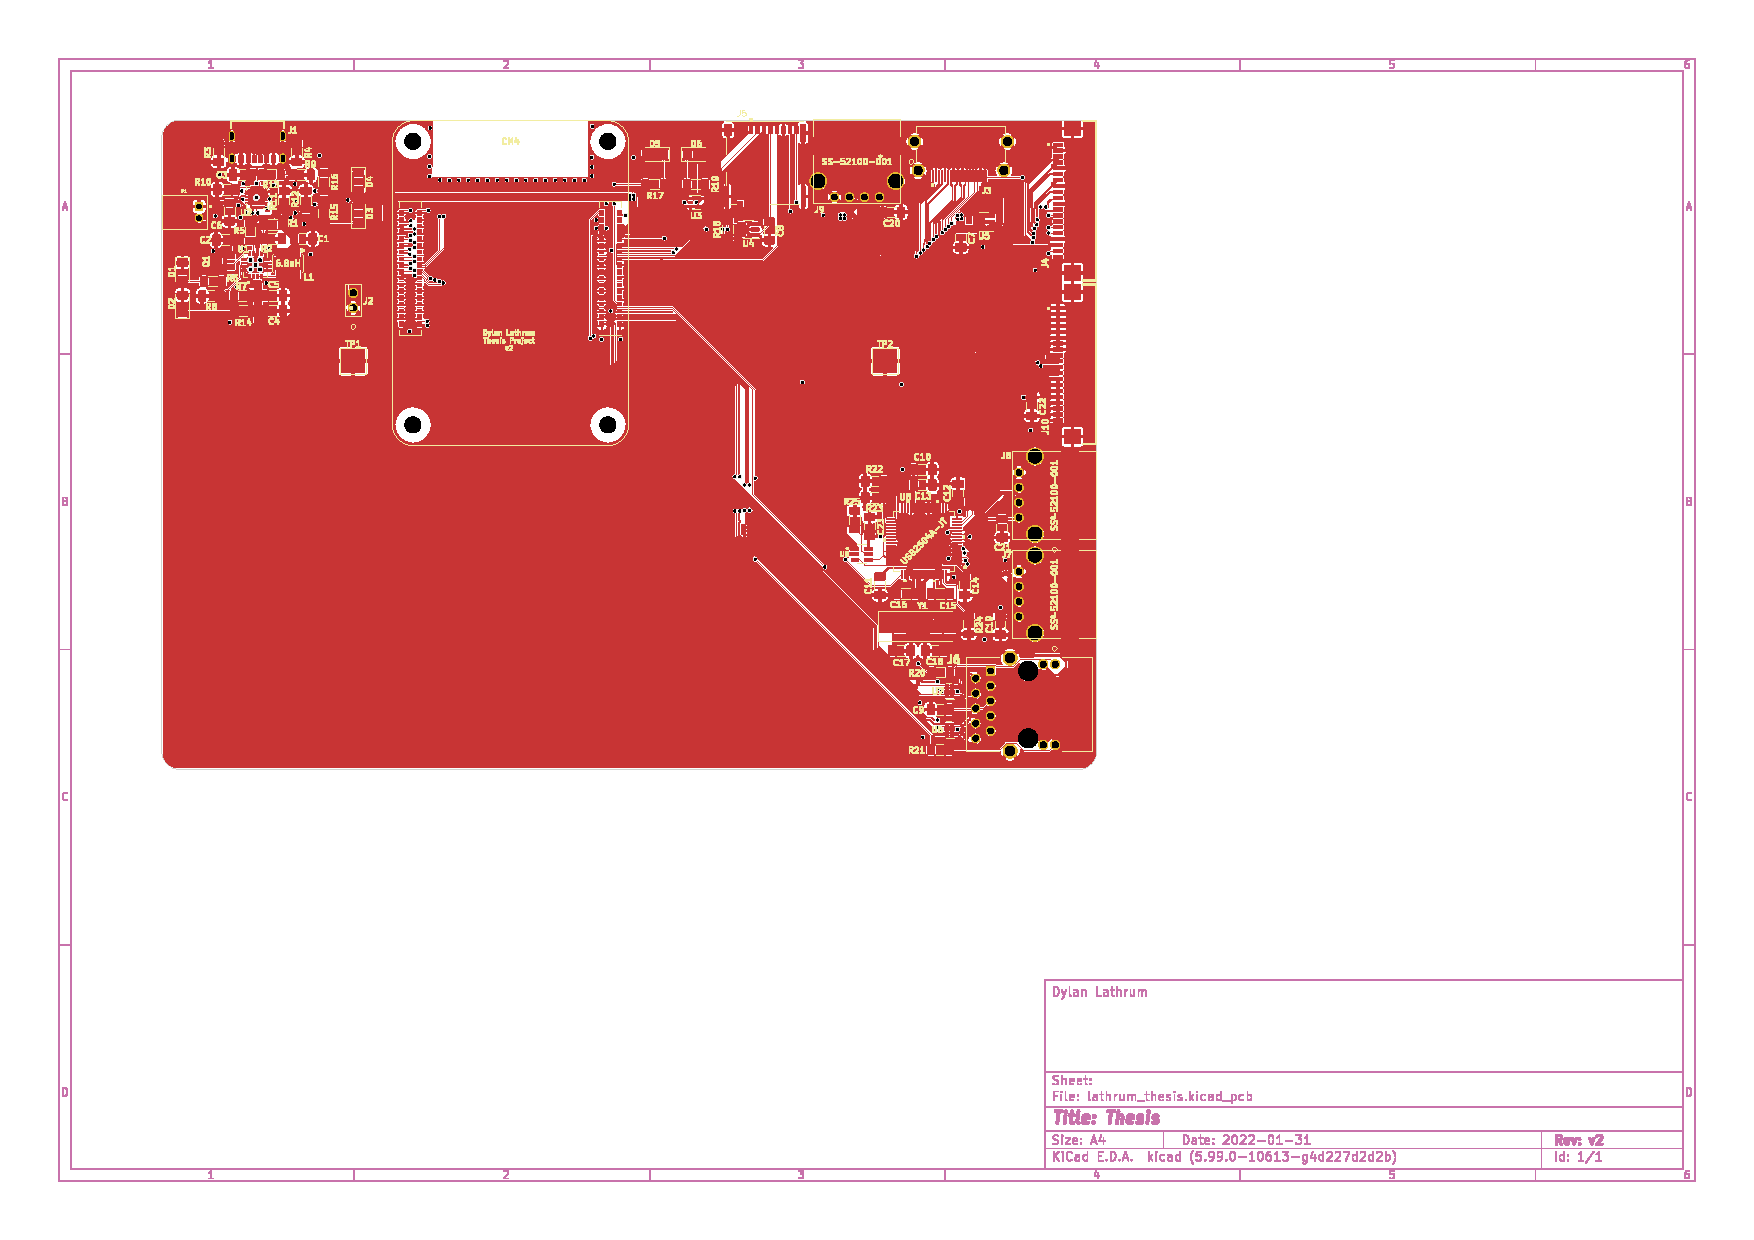
\includegraphics[height=0.9\textwidth,angle=90,page=1]{Figures/kicad/lathrum_thesis_layout_front.pdf}
  \captionsetup{width=.8\linewidth}
  \caption[PCB Front Layout]{Physical board layout for the front side of the PCB}
  \label{fig:pcb_layout_front}
\end{figure}

\begin{figure}[h]
  \centering
  %Height instead of width because the image is rotated
  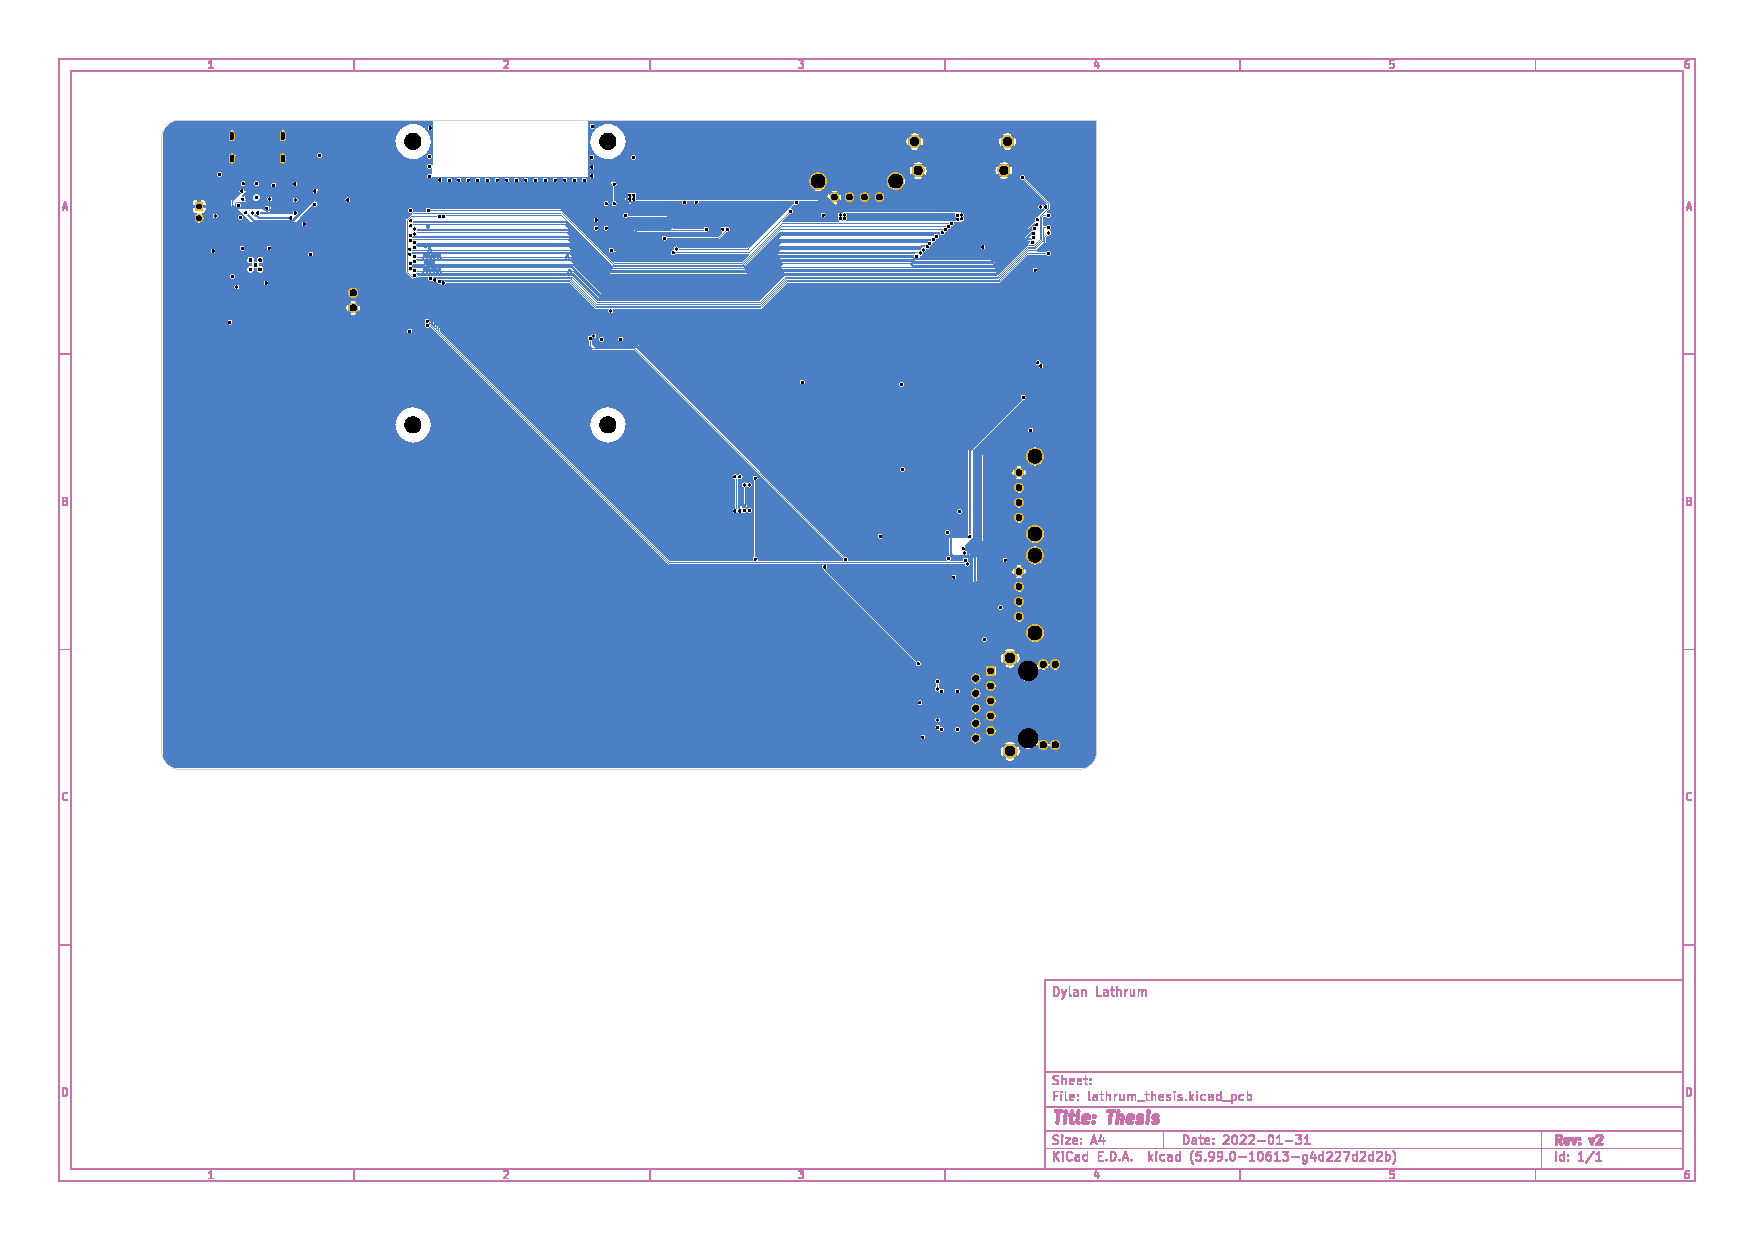
\includegraphics[height=0.9\textwidth,angle=90,page=1]{Figures/kicad/lathrum_thesis_layout_back.pdf}
  \captionsetup{width=.8\linewidth}
  \caption[PCB Back Layout]{Physical board layout for the back side of the PCB}
  \label{fig:pcb_layout_back}
\end{figure}